\chapter{Einleitung}
\section{Team}
\begin{figure}[htb]
	\centering
	\begin{minipage}{0.45\linewidth}
		\centering
		
\includegraphics[scale=0.5]{content/pictures/Florian.png}
		\caption{Florian Durli}
		\vspace{30pt}
	\end{minipage}
	\begin{minipage}{0.45\linewidth}
		\centering
		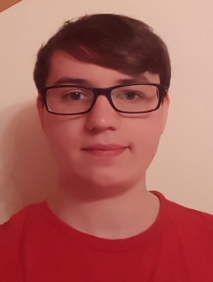
\includegraphics[scale=0.56]{content/pictures/Jannik.png}
		\caption{Jannik Ivosevic}
		\vspace{30pt}
	\end{minipage}
	\begin{minipage}{0.45\linewidth}
		\centering
		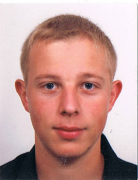
\includegraphics[scale=0.87]{content/pictures/Johannes.png}
		\caption{Johannes But}
		\vspace{30pt}
	\end{minipage}
	\begin{minipage}{0.45\linewidth}
		\centering
		
\includegraphics[scale=0.058]{content/pictures/Marco.jpeg}
		\caption{Marco Mayer}
		\vspace{30pt}
	\end{minipage}
	\begin{minipage}{0.45\linewidth}
		\centering
		
\includegraphics[scale=0.9]{content/pictures/Koray.jpg}
		\caption{Koray Ektekin}
		\vspace{30pt}
	\end{minipage}
\end{figure}
\section{Rollenverteilung}
\begin{table}[h]
\centering
	\begin{tabular}{l|l}
		\toprule
		\textbf{Phase}& \textbf{Projektleiter}\\
		\midrule
		Anforderungen & \docDritterReferent 	\\ 
		Implementation& \docErsterReferent	\\
		Test		  & \docZweiterReferent	\\ 
		Dokumentation \& Präsentation	& \docVierterReferent, \docFuenfterReferent\\
		\bottomrule
	\end{tabular}
	\caption{Rollenverteilung}
\end{table}
\noindent 
Der Projektleiter wechselt jede Phase. In der obigen Tabelle sind diese aufgeführt.
Der Projektleiter ist jeweils für die Koordination der Aufgaben und die
Organisation zuständig. Er dient als Ansprechpartner für das Projekt und gibt
eine „Fahrtrichtung“ vor. Jedoch werden sämtliche wichtige Entscheidungen
im Plenum getroffen. 
\section{Spielidee}
\subsection{Spielkonzept}
Unser Spiel namens „InfinityRun“ wird ein Endlos-Spiel sein bei der es das Ziel ist die Spielfigur so lange wie möglich am Leben zu erhalten. Der dazugehörige Highscore ist abhängig von der Lebensdauer der Spielfigur. Bei ansteigender Zeit wird die Geschwindigkeit des Spiels stetig erhöht. Das Spielfeld mit den Hindernissen wird per Zufallsgenerator erzeugt, somit ist jeder Durchlauf einzigartig. Spiel begleitend wird ein Soundtrack das Spielerlebnis abrunden. Bei Aufprall auf ein Hindernis, besteht die Möglichkeit das Spiel neu zu starten.
\newpage
\subsection{Entwurfsskizze}
\begin{figure}[htb]
	\centering
	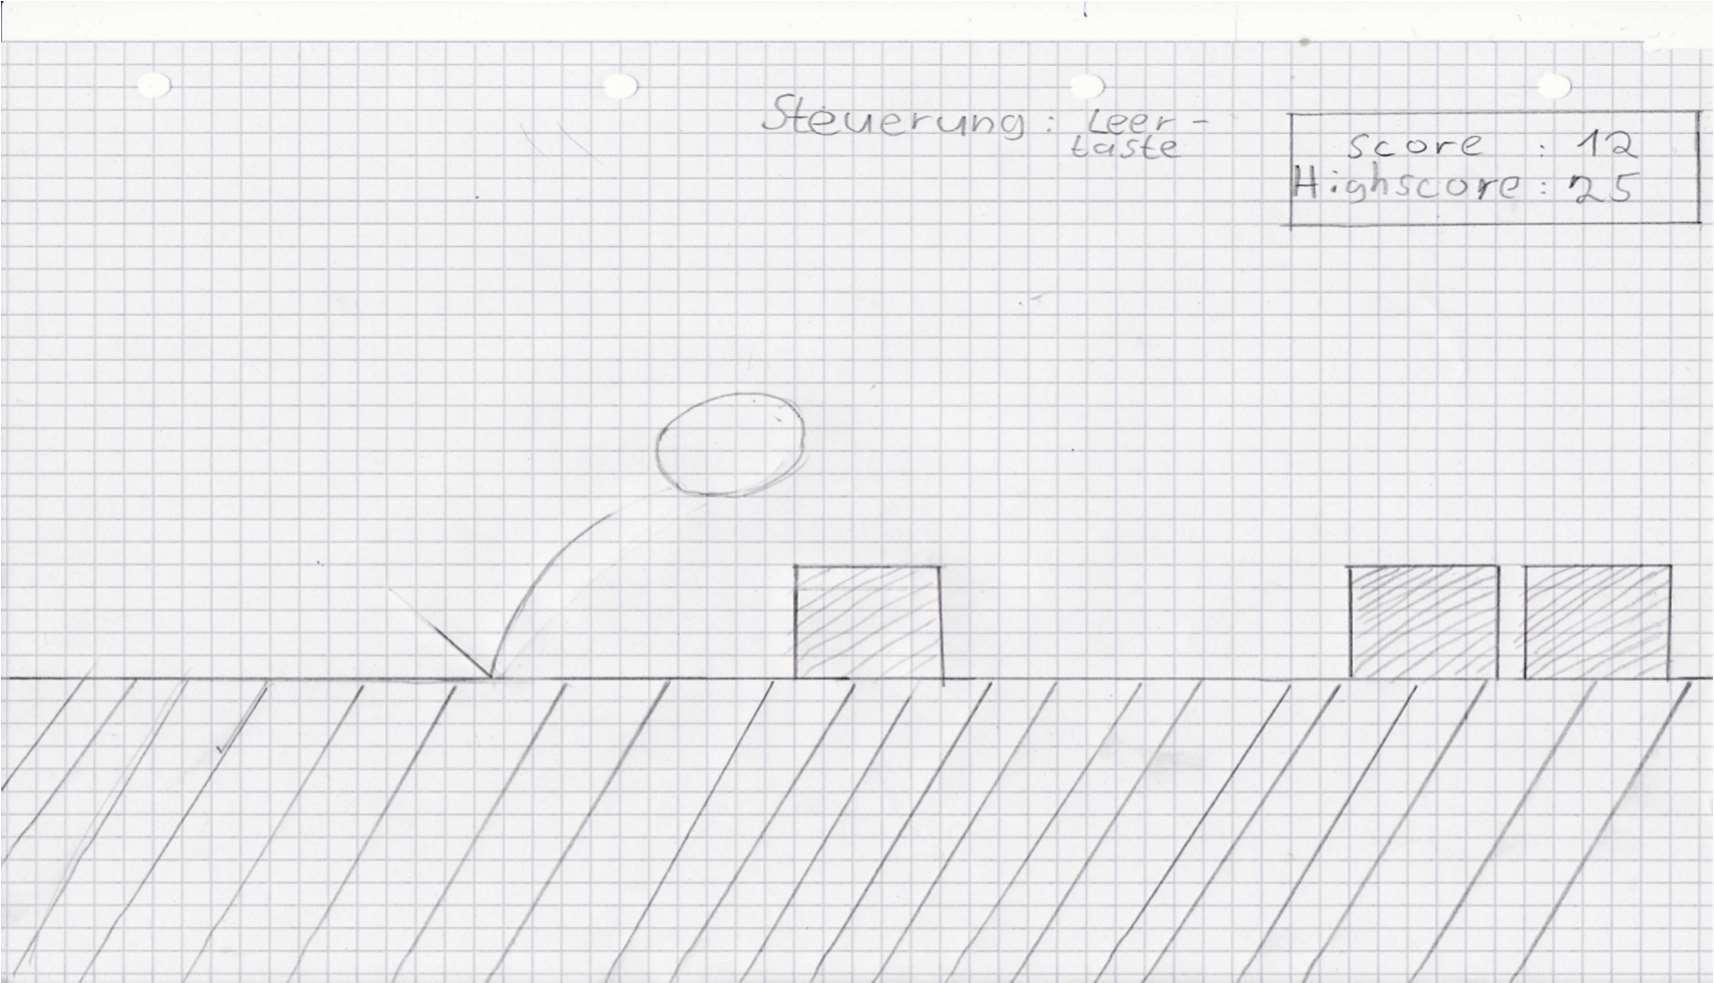
\includegraphics[scale=0.22]{content/pictures/entwurfsskizze.png}
	\caption{Entwurfsskizze}
\end{figure}
\noindent
Auf der abgebildeten Entwurfsskizze sehen sie die grobe Oberfläche unseres Spieles. Der V ähnliche Strich zeigt den Absprung eines Objektes, welches auf der Entwurfsskizze eine Kugel ist. Dies geschieht mit der Leertaste auf der Tastatur. Außerdem sind auf dem Bild noch verschiedene Blöcke zu sehen. Diese Blöcke werden Zufällig von rechts in den Bildschirm geniert. Es können verschieden Kombinationen z.B. ein Block, zwei Blöcke oder drei Blöcke generiert werden. Außerdem kann man oben im rechten Rand den Score und den jeweils erreichten Highscore sehen. In unserer Entwurfsskizze ist der Score 12 und der Highscore 25. Dieser sogenannte Score berechnet sich, je nachdem über wie viele Blöcke unser Objekt gesprungen ist. Ist er über einen Block und danach über drei Blöcke gesprungen zählt es nur zwei Punkte, da es nicht die Anzahl der Blöcke zählen soll, sondern die Anzahl der geschafften Sprünge. Der Highscore ist der jemals erreichte höchste Score in dem Spiel. Außerdem kann man neben dem Score und dem Highscore noch die Spielsteuerung sehen. Diese ist natürlich die Leertaste. Daneben soll noch ein Pausebutton sichtbar sein, womit man das Spiel pausieren kann. Dieser Pausebutton wird mit der Taste P hinterlegt. Man muss mit dem Objekt das richtige Timing erwischen, um über die Blöcke zu springen, anderenfalls landet man in einem oder mehreren Blöcken und darf nochmal von vorne beginnen. Um das Spiel interessanter zu gestalten wird das Spiel nach einem bestimmten Score schneller und somit schwieriger.
\newpage
\subsection{Erforderliche Software}
\subsubsection{Notepad++}
Notepad++ ist ein freier Editor der es ermöglicht die Syntax von JavaScript korrekt und mit Highlighting darzustellen. Dieser Editor wird immer beliebter durch seine Unterstützung verschiedener Programmiersprachen.
\subsubsection{Chrome}
Chrome ist ein Webbrowser von der Firma Google der immer populärer wird. Er ist besonders Benutzerfreundlich für Entwickler und bietet verschiedene Tools zum Debuggen.
\subsubsection{Gimp}
Zur erstellen unserer Grafiken benutzen wir das Bildbearbeitungsprogramm Gimp. Dies ist eine frei erhältliche Software, die einen erweiterten Funktionsumfang ähnlich wie das bekannte Programm Photoshop von Adobe bietet.
\subsubsection{Git/Github}
Wir haben uns dagegen entschieden die Softwareverwaltung der Hochschule zu nutzen und greifen nun auf eine alternative Lösung Namens Git zurück. Git ist eine freie Softwareverwaltung die von Linus Torvalds entstand. Github ist eine Open Source Plattform die dieses Konzept nutzt. Somit können wir parallel an dem Projekt arbeiten. Versionsstände definieren auf die wir jeder Zeit wieder zurück springen können. Somit ist ein Arbeiten wie in einem richtigen Softwareprojekt möglich.
